\chapter{معادلة شرودنغر والتوابع الموجية}\label{ch:b2:schrodinger-wave-functions}

أطلق الإلكترونات واحدًا واحدًا على شقّين وسجّل أين تقع كل
واحدة: نقطة هنا، ونقطة هناك، عشوائيًّا في الظاهر --- وبعد عشرة
آلاف نقطة، هدب تجربة يونغ، كأن كل إلكترون
مرّ من الشقّين معًا وتداخل مع نفسه. وقد لقي الفصل
الأخير من مجلد السنة الأولى هذه الغرابة: فالضوء يأتي في
فوتونات، وللمادة طول موجة $\lambda = h/p$، ولا يمكن أن يكون الموضع و
كمية الحركة حادّين معًا. وما لم يعطه هو
\emph{المعادلة} --- أي القاعدة التي تقول كيف تتطور الموجة المرافقة
لجسيم، كما يقول قانون نيوتن كيف يتطور مسار. وتلك
المعادلة هي معادلة شرودنغر (1926)، وبها يصير الوصف الكمومي
نظرية قابلة للحساب: إذ يُكتَب \emph{\omterm{def:b2:schrodinger-wave-functions:psi}{تابع موجي}}
$\psi(x,t)$، مربع طويلته احتمال إيجاد
الجسيم، وتُحلّ معادلة تفاضلية جزئية خطية. وهذا
الفصل يذكر المعادلة، ويفسّر ما تعنيه $\psi$ وما لا تعنيه،
ويجد حالاتها المستقرة ورزم الموجات للجسيم الحر،
ويبيّن أين يظهر ميكانيك نيوتن من جديد --- من أجل
كل ما هو أثقل من جزيء.

\begin{omfigure}
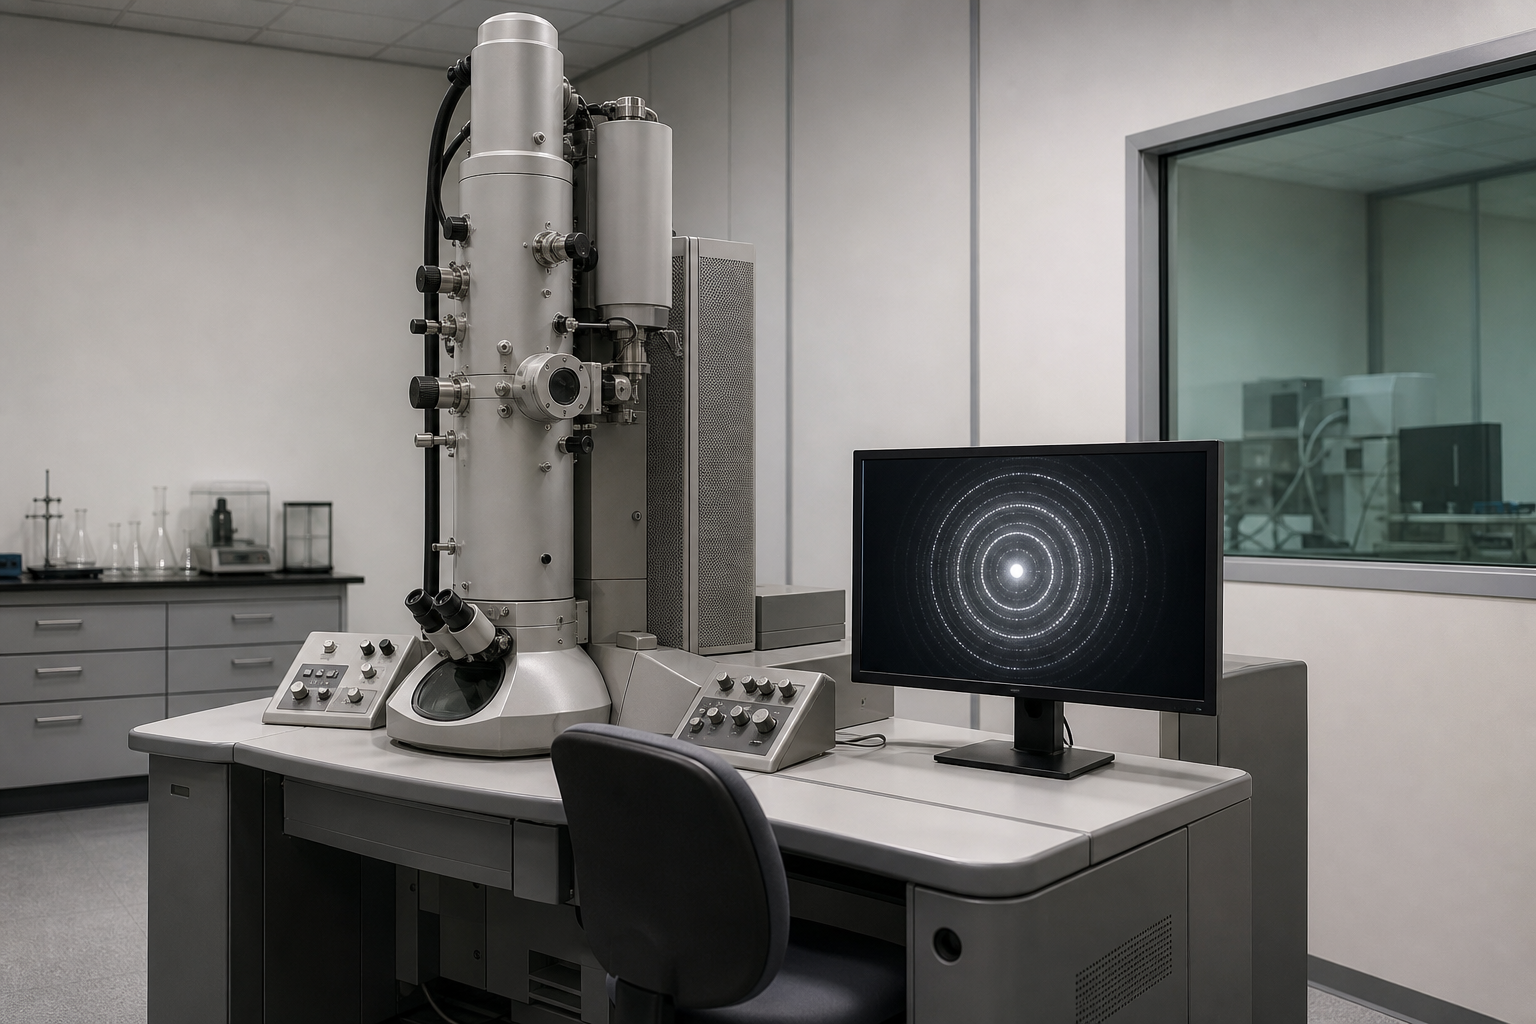
\includegraphics[width=0.58\linewidth]{images/book4/ai/b4-30-electron-microscope.png}

{\small مجهر إلكتروني نافذ: للإلكترونات المسرَّعة إلى
مئة كيلوفولط طول موجة قدره بضعة بيكومترات، ويصوّر تابعها
الموجي، مجمَّعًا بعدسات مغناطيسية، ذرات
بلورة.}
\end{omfigure}

\section{ما تركه لنا مجلد السنة الأولى}

\begin{proposition}[الجسيمات أمواج]\label{prop:b2:schrodinger-wave-functions:recap}
لفوتون تواتره $\nu$ الطاقة $E = h\nu = \hbar\omega$ وكمية
الحركة $p = h/\lambda = \hbar k$؛ والجسيم المادي الذي كمية حركته $p$
يتصرف موجةً طول موجتها $\lambda = h/p$ (دي برولي)، مع $E =
\hbar\omega$ و $p = \hbar k$ أيضًا --- \omterm{def:b2:diffraction:huygens}{وحيود} الإلكترونات على
البلورات، وقياس التداخل بالنترونات بل بالجزيئات يؤكد ذلك؛ ولا
حالة تكون فيها الموضع وكمية الحركة أحدّ من $\Delta x\,\Delta p
\ge \hbar/2$ (هايزنبرغ). ومع $\hbar = h/2\pi = \qty{1.05e-34}{J.s}$: لإلكترون
عند \qty{100}{eV} $\lambda = \qty{0.12}{nm}$، أي حجم
ذرة؛ ولحبيبة غبار \qty{1e-15}{kg} عند \qty{1}{mm/s} $\lambda =
\qty{7e-16}{m}$، أي أصغر من نواة --- فتتصرف تصرفًا كلاسيكيًّا.
\end{proposition}

\begin{proof}
مذكور من مجلد السنة الأولى؛ والمهمة الآن ديناميك
الموجة.
\end{proof}

\begin{omfigure}
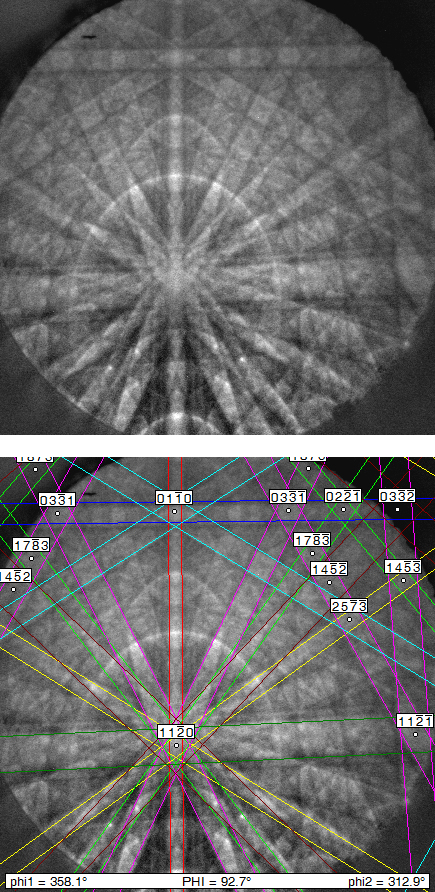
\includegraphics[width=0.4\linewidth, viewport=0 214 209 428, clip]{images/book4/electron-diffraction-nist.jpg}

{\small نقش \omterm{def:b2:diffraction:huygens}{حيود} إلكتروني مسجَّل في مجهر إلكتروني (وهو نقش كيكوتشي من بلورة): إلكترونات طول موجتها بضعة بيكومترات، محيدة على المستويات الذرية --- أي المادة تتصرف موجةً (المعهد الوطني الأمريكي للمعايير والتقانة).}
\end{omfigure}

\section{التابع الموجي}

\begin{definition}[التابع الموجي وقاعدة بورن]\label{def:b2:schrodinger-wave-functions:psi}
تُوصَف حالة جسيم يتحرك وفق $x$ بواسطة \emph{تابع موجي}\index{تابع موجي}
عقدي $\psi(x,t)$ بحيث يكون
\[
\dd\mathcal P = |\psi(x,t)|^2\,\dd x
\]
احتمال إيجاد الجسيم بين $x$ و $x + \dd x$
عند اللحظة $t$ (وهي \emph{قاعدة بورن}\index{قاعدة بورن})؛ ومن ثَمّ
\emph{التنظيم} $\int_{-\infty}^{\infty}|\psi|^2\dd x = 1$، و
القيم المتوقعة $\langle x\rangle = \int x|\psi|^2\dd x$، و $\Delta x^2 =
\langle x^2\rangle - \langle x\rangle^2$. والتوابع الموجية تحقق
\emph{مبدأ التراكب}\index{مبدأ التراكب}: فإذا كانت
$\psi_1$ و $\psi_2$ حالتين ممكنتين، كانت $\alpha\psi_1 +
\beta\psi_2$ كذلك (منظَّمةً)، وتحوي الاحتمالات عندئذ
حدّ التداخل $2\operatorname{Re}(\alpha^*\beta\,\psi_1^*\psi_2)$. وعامل
الطور الشامل $\eu^{\iu\theta}$ لا يغيّر شيئًا؛ أما الطور النسبي
بين مركّبتين متراكبتين فيغيّر التداخل.
\end{definition}

\begin{remark}[ما ليست $\psi$]\label{rem:b2:schrodinger-wave-functions:not}
ليست $\psi$ حقلًا كلاسيكيًّا منتشرًا في الفضاء مثل $\vect E$، ولا
غيمة مادة: فالإلكترون يوجد دائمًا كاملًا، في نقطة واحدة.
و $\psi$ \emph{سعة احتمال}، وهي الشيء الذي
يتداخل؛ ولا يُرصَد إلا $|\psi|^2$، ولا إحصائيًّا إلا،
بتكرار التجربة على جسيمات محضَّرة تحضيرًا متطابقًا. ونقاط
الشقّين إلكترونات مفردة؛ والهدب هي $|\psi_1 +
\psi_2|^2$.
\end{remark}

\section{معادلة شرودنغر}

\begin{theorem}[معادلة شرودنغر]\label{thm:b2:schrodinger-wave-functions:equation}
لجسيم كتلته $m$ في طاقة كامنة $V(x)$ \omterm{def:b2:schrodinger-wave-functions:psi}{تابع
موجي} يحقق
\[
\iu\hbar\,\frac{\partial\psi}{\partial t} = -\frac{\hbar^2}{2m}\,\frac{\partial^2\psi}{\partial x^2} + V(x)\,\psi .
\]
وهي خطية (فالتراكب)، ومن المرتبة الأولى في الزمن (\omterm{def:b2:schrodinger-wave-functions:psi}{فالتابع الموجي}
عند لحظة يحدده في كل اللحظات التالية)، وعقدية ($\psi$
لا يمكن أن تكون حقيقية: فالوحدة التخيلية $\iu$ جوهرية). وهي \emph{مصادرة}،
تبرّرها نتائجها.
\end{theorem}

\begin{proof}
تسويغ لا برهان. فالجسيم الحرّ ذو كمية الحركة الحادّة
$p = \hbar k$ والطاقة $E = \hbar\omega$ ينبغي أن يكون موجة مستوية $\psi =
A\eu^{\iu(kx - \omega t)}$، ولها $\iu\hbar\partial_t\psi = \hbar\omega\psi =
E\psi$ و $-(\hbar^2/2m)\partial_x^2\psi = (\hbar^2k^2/2m)\psi = (p^2/2m)\psi$.
فالعلاقة الكلاسيكية $E = p^2/2m$ تعيد إنتاجها المعادلة
$\iu\hbar\partial_t\psi = -(\hbar^2/2m)\partial_x^2\psi$، والتعميم
الطبيعي من أجل $E = p^2/2m + V$ يضيف $V\psi$. ولاحظ أن
المعادلة يجب أن تكون خطية لتصحّ من أجل تراكبات الأمواج المستوية، و
من المرتبة الأولى في الزمن مع $\iu$ حتى يكون $\eu^{-\iu\omega t}$ لا
$\cos\omega t$ هو التعلق بالزمن --- إذ كانت معادلة أمواج حقيقية
تعطي $E^2 \propto p^4$.
\end{proof}

\begin{proposition}[حفظ الاحتمال]\label{prop:b2:schrodinger-wave-functions:current}
كثافة الاحتمال $\rho = |\psi|^2$ و\emph{تيار
الاحتمال}\index{تيار الاحتمال}
\[
j = \frac{\hbar}{m}\operatorname{Im}\Big(\psi^*\frac{\partial\psi}{\partial x}\Big)
= \frac{\hbar}{2\iu m}\Big(\psi^*\partial_x\psi - \psi\,\partial_x\psi^*\Big)
\]
يحققان $\partial_t\rho + \partial_xj = 0$: فالاحتمال لا يُحدَث ولا
يُتلَف، ويبقى $\int|\psi|^2\dd x$ مساويًا $1$. ومن أجل موجة مستوية
$A\eu^{\iu kx}$، $j = |A|^2\hbar k/m = \rho v$: أي الكثافة في السرعة، كما في
أي جريان.
\end{proposition}

\begin{proof}
$\partial_t(\psi^*\psi) = \psi^*\partial_t\psi + \psi\,\partial_t\psi^*$؛ ومن
المعادلة ومرافقتها، $\partial_t\psi = (\iu\hbar/2m)\partial_x^2\psi -
(\iu/\hbar)V\psi$، و $\partial_t\psi^* = -(\iu\hbar/2m)\partial_x^2\psi^* +
(\iu/\hbar)V\psi^*$؛ فيُختصر حدّا $V$ والباقي هو $(\iu\hbar/2m)(\psi^*
\partial_x^2\psi - \psi\,\partial_x^2\psi^*) = -\partial_xj$.
\end{proof}

\begin{proposition}[كمية الحركة والقيم المتوقعة والحدّ الكلاسيكي]\label{prop:b2:schrodinger-wave-functions:ehrenfest}
تُنال كمية حركة حالة بالمؤثر $\hat p =
-\iu\hbar\,\partial_x$ (الذي يعطي $\hbar k$ على موجة مستوية): $\langle
p\rangle = \int\psi^*(-\iu\hbar\partial_x\psi)\dd x$، وتُنال الطاقة بالمؤثر $\hat H
= -(\hbar^2/2m)\partial_x^2 + V$. والقيم المتوقعة تحقق
(إهرنفست)
\[
\frac{\dd\langle x\rangle}{\dd t} = \frac{\langle p\rangle}{m}, \qquad
\frac{\dd\langle p\rangle}{\dd t} = -\Big\langle\frac{\dd V}{\dd x}\Big\rangle :
\]
فمركز \omterm{prop:b2:schrodinger-wave-functions:free}{رزمة الموجة} يتبع قانون نيوتن بالضبط حين تكون $V$
تربيعية على الأكثر، وبالتقريب متى كانت الرزمة ضيقة
بالقياس إلى السلّم الذي تتغير عليه $V$ --- وهو الحدّ الكلاسيكي،
وهو يصحّ من أجل أي جسم عياني لأن $\hbar$ صغيرة إلى هذا الحدّ.
\end{proposition}

\begin{proof}
اشتقّ $\langle x\rangle = \int x|\psi|^2$، واستعمل $\partial_t\rho =
-\partial_xj$ وكامِل بالتجزئة: $\dd\langle x\rangle/\dd t = \int j\,\dd x
= \langle p\rangle/m$. والعلاقة الثانية هي الحساب نفسه من
مرتبة أعلى (وهو مقبول هنا).
\end{proof}

\section{الحالات المستقرة}

\begin{theorem}[الحالات المستقرة]\label{thm:b2:schrodinger-wave-functions:stationary}
إذا لم تتعلق $V$ بالزمن، كانت للمعادلة حلول من الشكل
المفصول
\[
\psi(x,t) = \varphi(x)\,\eu^{-\iu Et/\hbar}, \qquad
-\frac{\hbar^2}{2m}\,\varphi'' + V\varphi = E\varphi
\]
(وهي \emph{معادلة شرودنغر المستقلة عن الزمن}\index{معادلة شرودنغر!المستقلة
عن الزمن}): أي \emph{الحالات المستقرة}\index{حالة
مستقرة}، ذات الطاقة المعيَّنة $E$، وكثافة احتمالها
$|\varphi|^2$ لا تتحرك. والطاقات $E$ التي تكون $\varphi$ من أجلها
مقبولة (محدودة، وقابلة للتنظيم في حالة مرتبطة) هي
\emph{مستويات الطاقة}؛ والحلّ العام تراكب $\psi =
\sum_nc_n\varphi_n(x)\eu^{-\iu E_nt/\hbar}$، ولتراكب مستويين
كثافة تتذبذب عند \emph{تواتر بور}\index{تواتر
بور} $\nu_{21} = (E_2 - E_1)/h$ --- وهو تواتر الضوء الذي
تصدره الذرة أو تمتصّه.
\end{theorem}

\begin{proof}
عوّض $\varphi(x)f(t)$: $\iu\hbar f'/f = (-\hbar^2\varphi''/2m + V\varphi)/\varphi$،
أي تابع في $t$ يساوي تابعًا في $x$، فهو ثابت $E$؛ و $f
= \eu^{-\iu Et/\hbar}$. ومن أجل مستويين، $|c_1\varphi_1\eu^{-\iu E_1t/\hbar} +
c_2\varphi_2\eu^{-\iu E_2t/\hbar}|^2 = |c_1\varphi_1|^2 + |c_2\varphi_2|^2 +
2\operatorname{Re}(c_1^*c_2\varphi_1^*\varphi_2\eu^{-\iu(E_2 - E_1)t/\hbar})$.
وتمام \omterm{thm:b2:schrodinger-wave-functions:stationary}{الحالات المستقرة} مقبول.
\end{proof}

\begin{omfigure}
\begin{tikzpicture}
  \begin{axis}[omaxis, width=7.4cm, height=4.4cm, xmin=0, xmax=1, ymin=-1.3, ymax=1.5,
    xlabel={$x/L$}, ylabel={$\psi$}, xtick={0.5,1}, ytick=\empty, clip=false,
    legend style={font=\scriptsize, at={(0.5,-0.28)}, anchor=north, draw=none, fill=none, legend columns=3}]
    \addplot[omDef, thick, domain=0:1, samples=80] {1.41*sin(deg(pi*x))*cos(40)};
    \addlegendentry{$\operatorname{Re}\psi$}
    \addplot[omExo, thick, dashed, domain=0:1, samples=80] {-1.41*sin(deg(pi*x))*sin(40)};
    \addlegendentry{$\operatorname{Im}\psi$}
    \addplot[omThm, thick, domain=0:1, samples=80] {2*sin(deg(pi*x))^2-1.3};
    \addlegendentry{$|\psi|^2$ (مزاح)}
  \end{axis}
  \begin{scope}[xshift=9.4cm, yshift=1.3cm, >=stealth]
    \draw[->] (-1.5,0) -- (1.5,0) node[right, font=\scriptsize] {حقيقي};
    \draw[->] (0,-1.5) -- (0,1.5) node[above, font=\scriptsize] {تخيلي};
    \draw[gray] (0,0) circle (1.1);
    \draw[->, omDef, very thick] (0,0) -- (-40:1.1);
    \draw[->, omDef] (1.1,0) arc (0:-40:1.1);
    \node[font=\scriptsize, omDef] at (-50:1.55) {$-Et/\hbar$};
    \node[font=\scriptsize] at (0,-1.85) {$\eu^{-\iu Et/\hbar}$};
  \end{scope}
\end{tikzpicture}

{\small \omterm{thm:b2:schrodinger-wave-functions:stationary}{حالة مستقرة}: المقطع المكاني $\varphi(x)$ (وهو هنا
الحالة الأساسية لبئر) مضروبًا في \omterm{thm:b2:gratings:nwaves}{شعاع طوري} يدور بالمعدل
$E/\hbar$؛ فيدور الجزآن الحقيقي والتخيلي أحدهما في الآخر بينما
يقف $|\psi|^2$.}
\end{omfigure}

\begin{omfigure}
\begin{tikzpicture}
  \begin{axis}[omaxis, width=9cm, height=4.4cm, xmin=0, xmax=1, ymin=0, ymax=2.6,
    xlabel={$x/L$}, ylabel={$|\psi|^2$}, xtick={0.5,1}, ytick=\empty, clip=false,
    legend style={font=\scriptsize, at={(0.5,-0.28)}, anchor=north, draw=none, fill=none, legend columns=3}]
    \addplot[omDef, thick, domain=0:1, samples=100] {(sin(deg(pi*x)))^2 + (sin(deg(2*pi*x)))^2 + 2*sin(deg(pi*x))*sin(deg(2*pi*x))};
    \addlegendentry{$t = 0$}
    \addplot[omThm, thick, dashed, domain=0:1, samples=100] {(sin(deg(pi*x)))^2 + (sin(deg(2*pi*x)))^2};
    \addlegendentry{$t = T_{21}/4$}
    \addplot[omExo, thick, domain=0:1, samples=100] {(sin(deg(pi*x)))^2 + (sin(deg(2*pi*x)))^2 - 2*sin(deg(pi*x))*sin(deg(2*pi*x))};
    \addlegendentry{$t = T_{21}/2$}
  \end{axis}
\end{tikzpicture}

{\small تراكب أدنى حالتين في بئر: تتمايل
الكثافة من جهة إلى أخرى عند \omterm{thm:b2:schrodinger-wave-functions:stationary}{تواتر بور}
$(E_2 - E_1)/h$ --- أي شحنة متذبذبة، ومن ثَمّ (\cref{ch:b2:dipole-radiation})
ثنائي قطب مشعّ عند تواتر الخط الطيفي بالضبط.}
\end{omfigure}

\section{الجسيم الحرّ: الأمواج المستوية ورزم الموجات}

\begin{proposition}[الجسيم الحرّ]\label{prop:b2:schrodinger-wave-functions:free}
من أجل $V = 0$ تكون \omterm{thm:b2:schrodinger-wave-functions:stationary}{الحالات المستقرة} هي الأمواج المستوية $\eu^{\iu(kx -
\omega t)}$ مع
\[
E = \hbar\omega = \frac{\hbar^2k^2}{2m}, \qquad
v_\varphi = \frac{\omega}{k} = \frac{\hbar k}{2m}, \qquad
v_{\text{g}} = \frac{\dd\omega}{\dd k} = \frac{\hbar k}{m} = \frac{p}{m} :
\]
فأمواج المادة \emph{مبدِّدة}؛ وليس \omterm{def:b2:dispersion-wave-packets:relation}{لسرعة الطور} معنى
فيزيائي، و\emph{\omterm{prop:b2:dispersion-wave-packets:group}{سرعة المجموعة}} هي سرعة الجسيم. والموجة المستوية
غير قابلة للتنظيم --- إذ الجسيم ذو كمية الحركة الحادّة تمامًا
منتشر على الفضاء كله --- ومن ثَمّ فالجسيم الحقيقي \emph{رزمة
موجة}\index{رزمة موجة}، أي تراكب أمواج مستوية على نطاق
$\Delta k$، موضَّعة على $\Delta x \sim 1/\Delta k$، تتحرك بالسرعة $v_{\text{g}}$ و
\emph{تنتشر}: فرزمة غاوسية عرضها الابتدائي $\sigma_0$ لها عند
اللحظة $t$ العرض
\[
\sigma(t) = \sigma_0\sqrt{1 + \Big(\frac{\hbar t}{2m\sigma_0^2}\Big)^2}, \qquad
\tau = \frac{2m\sigma_0^2}{\hbar} ,
\]
وتحقق $\Delta x\,\Delta p = \hbar/2$ عند $t = 0$ (وهو الأصغر المسموح)
وأكثر منه لاحقًا.
\end{proposition}

\begin{proof}
تنتج \omterm{def:b2:dispersion-wave-packets:relation}{علاقة التبدد} من المعادلة؛ و $v_{\text{g}}$ كما في
\cref{ch:b2:dispersion-wave-packets}. وتأتي صيغة الانتشار من
تركيب فورييه للرزمة --- إذ تلتقط كل مركّبة $\eu^{\iu kx}$
الطور $\eu^{-\iu\hbar k^2t/2m}$، ويعطي التكامل الغاوسي بمعامل
عقدي غاوسيًّا متزايد العرض؛ وتكامل فورييه أداة
مجلد رياضيات السنة الثالثة ونقبل
النتيجة. وأما فيزيائيًّا: فالرزمة تحوي كميات حركة منتشرة على $\Delta p
= \hbar/2\sigma_0$، ومن ثَمّ سرعات منتشرة على $\Delta v = \hbar/2m\sigma_0$،
وبعد $t$ تكون المركّبات الأسرع قد سبقت الأبطأ بالمقدار $\Delta v\,t$
--- وهذا ما تقوله الصيغة بالضبط.
\end{proof}

\begin{omfigure}
\begin{tikzpicture}
  \begin{axis}[omaxis, width=6.2cm, height=4.4cm, xmin=0, xmax=3, ymin=0, ymax=2.6,
    xlabel={$k$}, ylabel={$\omega$}, xtick=\empty, ytick=\empty, clip=false]
    \addplot[omDef, thick, domain=0:2.3, samples=60] {x*x/2};
    \addplot[omExo, dashed, domain=0.4:2.6] {1.5*x-1.125};
    \addplot[omThm, dashed, domain=0:2.8] {0.75*x};
    \fill (axis cs:1.5,1.125) circle (1.5pt);
    \node[font=\scriptsize, omExo, anchor=west] at (axis cs:0.15,2.5) {$v_{\text{g}} = \hbar k/m$ (المماس)};
    \node[font=\scriptsize, omThm, anchor=west] at (axis cs:2.3,1.5) {$v_\varphi = \hbar k/2m$};
    \node[font=\scriptsize] at (axis cs:0.8,1.5) {$\omega = \hbar k^2/2m$};
  \end{axis}
  \begin{axis}[omaxis, width=7cm, height=4.4cm, xmin=-2.5, xmax=10, ymin=0, ymax=1.15, xshift=6.8cm,
    xlabel={$x/\sigma_0$}, ylabel={$|\psi|^2$}, xtick=\empty, ytick=\empty, clip=false]
    \addplot[omDef, thick, domain=-2.5:10, samples=120] {exp(-(x-1)^2/2)};
    \addplot[omThm, thick, domain=-2.5:10, samples=120] {(1/1.41)*exp(-(x-3.5)^2/4)};
    \addplot[omExo, thick, domain=-2.5:10, samples=120] {(1/2.24)*exp(-(x-6)^2/10)};
    \node[font=\scriptsize, omDef, anchor=west] at (axis cs:1.3,1.0) {$t = 0$};
    \node[font=\scriptsize, omThm, anchor=west] at (axis cs:3.8,0.75) {$\tau$};
    \node[font=\scriptsize, omExo, anchor=west] at (axis cs:6.3,0.5) {$2\tau$};
  \end{axis}
\end{tikzpicture}

{\small على اليسار: منحني تبدد الجسيم الحرّ، مع \omterm{prop:b2:dispersion-wave-packets:group}{سرعة
المجموعة} (وهي المماس) \omterm{def:b2:dispersion-wave-packets:relation}{وسرعة الطور} (وهي الوتر إلى المبدأ)، وهي نصفها.
وعلى اليمين: رزمة غاوسية تتحرك بالسرعة $v_{\text{g}}$ وتنتشر
--- وعرضها أكبر بالعامل $\sqrt2$ بعد $\tau = 2m\sigma_0^2/\hbar$، وقمتها
أدنى، ومساحتها ثابتة.}
\end{omfigure}

\begin{example}[من ينتشر]\label{ex:b2:schrodinger-wave-functions:spreading}
إلكترون موضَّع ضمن $\sigma_0 = \qty{1}{nm}$: $\tau = 2m\sigma_0^2/\hbar
= \qty{1.7e-14}{s}$ --- فبعد نانوثانية تصير رزمته بعرض \qty{60}{\micro m}:
فالإلكترون المتروك وحده لا يبقى في مكانه؛ وهو مرتبطًا في ذرة
لا ينتشر لأن الكمون يمسكه (أي \omterm{thm:b2:schrodinger-wave-functions:stationary}{حالة مستقرة}).
وحبيبة غبار \qty{1e-15}{kg} موضَّعة في \qty{1}{\micro m}: $\tau =
\qty{2e7}{s}$، أي ثمانية أشهر؛ ورصاصة: أطول من عمر الكون.
فالانتشار الكمومي حقيقي، وغير مرئي في كل ما يمكن رؤيته.
\end{example}

\begin{remark}[الطاقة والزمن]\label{rem:b2:schrodinger-wave-functions:energytime}
الحالة التي لا توجد إلا خلال $\Delta t$ --- كذرة مثارة عمرها
$\tau$، أو \omterm{prop:b2:scalar-light-model:coherence}{قطار موجة} طوله $c\tau$ --- تراكب طاقات
منتشرة على $\Delta E \sim \hbar/\Delta t$: أي علاقة فورييه في
\cref{ch:b2:scalar-light-model} بين مدة قطار وعرضه
الطيفي، مطبَّقةً الآن على $E = \hbar\omega$. ولمستوٍ ذري
عمره \qty{10}{ns} عرض $\Delta E = \qty{7e-8}{eV}$، أي عرض خط طبيعي
قدره \qty{16}{MHz}؛ وعرض دوبلر في \cref{ch:b2:laser}
(\qty{1.5}{GHz}) يخفيه في غاز، لا في ذرة باردة أو شاردة
ساكنة.
\end{remark}

\begin{method}[العمل بالتوابع الموجية]\label{meth:b2:schrodinger-wave-functions:method}
(1) نظِّم؛ والاحتمالات هي $\int|\psi|^2$ على المنطقة. (2)
ومع $V$ مستقلة عن الزمن: ابحث عن $\varphi(x)\eu^{-\iu Et/\hbar}$، وحلّ
المعادلة المستقرة، وافرض الشروط الحدية --- فالمستويات.
(3) وتراكَب \omterm{thm:b2:schrodinger-wave-functions:stationary}{الحالات المستقرة} من أجل التطور؛ ومستويان يضربان عند
$(E_2 - E_1)/h$. (4) والحركة الحرة: $v_{\text{g}} = p/m$، وزمن الانتشار
$2m\sigma_0^2/\hbar$. (5) والتيارات: $j = (\hbar/m)\operatorname{Im}(\psi^*\psi')$؛
ومن أجل $A\eu^{\iu kx} + B\eu^{-\iu kx}$، $j = (|A|^2 - |B|^2)\hbar k/m$ (بلا حدّ متقاطع).
(6) والحدّ الكلاسيكي: إهرنفست، و $\lambda$ في وجه حجم
الجهاز.
\end{method}

\section{تمارين}

\begin{exercise}[$\star$]\label{exo:b2:schrodinger-wave-functions:1}
أطوال موجة دي برولي: لإلكترون عند \qty{100}{eV}، و \qty{10}{keV}،
و \qty{100}{keV} (استعمل $p = \sqrt{2mE}$، ثم قل لمَ يحتاج الأخير إلى
تصحيح)؛ ولنترون حراري (\qty{25}{meV}، و $m = \qty{1.67e-27}{kg}$)؛ ولجزيء
C$_{60}$ ($m = \qty{1.2e-24}{kg}$) عند \qty{200}{m/s}؛ ولكرة
تنس. فأيّها يُظهر تداخلًا؟
\end{exercise}

\begin{exercise}[$\star$]\label{exo:b2:schrodinger-wave-functions:2}
$\psi(x) = A\eu^{-x^2/2a^2}$: أوجد $A$ (استعمل $\int\eu^{-u^2}\dd u = \sqrt\pi$)؛
و $\langle x\rangle$، و $\Delta x$؛ واحتمال إيجاد الجسيم في
$|x| < a$ ($\operatorname{erf}(1) = 0.84$) وفي $|x| < 2a$ ($0.9995$).
\end{exercise}

\begin{exercise}[$\star$]\label{exo:b2:schrodinger-wave-functions:3}
تحقق من أن $\varphi(x)\eu^{-\iu Et/\hbar}$ يحلّ المعادلة حين تحلّ $\varphi$
المستقرةَ. وأوجد تواتر \omterm{thm:b2:gratings:nwaves}{الشعاع الطوري} من أجل $E = \qty{1}{eV}$؛
ومن أجل تراكب مستويين بينهما \qty{2}{eV}، أوجد تواتر تذبذب $|\psi|^2$
وطول موجته --- وتواتر الضوء
المصدَر وطوله.
\end{exercise}

\begin{exercise}[$\star$]\label{exo:b2:schrodinger-wave-functions:4}
أوجد زمن الانتشار $\tau = 2m\sigma_0^2/\hbar$ والعرض بعد \qty{1}{ns} وبعد
\qty{1}{s}: من أجل إلكترون مع $\sigma_0 = \qty{1}{nm}$ و $\sigma_0 = \qty{1}{mm}$؛
وبروتون مع $\sigma_0 = \qty{1}{nm}$؛ وحبيبة \qty{1e-12}{kg} مع
$\sigma_0 = \qty{1}{\micro m}$. ولمَ تبقى الأجسام حيث تُوضَع؟
\end{exercise}

\begin{exercise}[$\star\star$]\label{exo:b2:schrodinger-wave-functions:5}
\emph{التيار.} (أ) استنتج \omterm{thm:b2:fluid-kinematics:continuity}{معادلة الاستمرار}. (ب) وأوجد $j$ من أجل
$A\eu^{\iu kx}$، ومن أجل $A\sin kx$، ومن أجل $A\eu^{\iu kx} + B\eu^{-\iu kx}$. (ج) ولمَ يكون
غياب الحدّ المتقاطع في الحالة الأخيرة قولًا بأن
التدفقين المنعكس والوارد يتطارحان لا غير؟ (د) وبيّن أن $j = 0$ من أجل \omterm{def:b2:schrodinger-wave-functions:psi}{تابع
موجي} حقيقي: \omterm{thm:b2:schrodinger-wave-functions:stationary}{فالحالة المستقرة} المرتبطة لا تحمل تيارًا.
\end{exercise}

\begin{exercise}[$\star\star$]\label{exo:b2:schrodinger-wave-functions:6}
\emph{رزمة غاوسية.} $\psi(x,0) = A\eu^{\iu k_0x}\eu^{-x^2/4\sigma^2}$. (أ)
أوجد $A$، و $\langle x\rangle$، و $\Delta x$. (ب) و $\langle p\rangle$ مع $\hat p =
-\iu\hbar\partial_x$. (ج) وبقبول $\Delta p = \hbar/2\sigma$، تحقق من
$\Delta x\Delta p = \hbar/2$. (د) وبرهن $\dd\langle x\rangle/\dd t = \langle
p\rangle/m$ من \omterm{thm:b2:fluid-kinematics:continuity}{معادلة الاستمرار}.
\end{exercise}

\begin{exercise}[$\star\star$]\label{exo:b2:schrodinger-wave-functions:7}
\emph{إلكترونات في أنبوب.} إلكترونات مسرَّعة عبر \qty{100}{V}
تقطع \qty{30}{cm}. (أ) أوجد السرعة وطول الموجة وزمن الطيران. (ب) والسرعتين
الطورية والزمرية؛ فأيّهما سرعة الإلكترون؟ (ج) ورزمة عرضها ابتداءً
\qty{10}{\micro m}: أوجد زمن الانتشار والعرض عند الوصول. (د) \omterm{def:b2:diffraction:huygens}{والحيود}
على فتحة \qty{0.3}{mm} في الطريق: أوجد الانتشار الزاوي والبقعة على
الشاشة. أتصحّ صورة الأشعة؟
\end{exercise}

\begin{exercise}[$\star\star$]\label{exo:b2:schrodinger-wave-functions:8}
\emph{الأطوار.} (أ) بيّن أن $\psi$ و $\eu^{\iu\theta}\psi$ تعطيان التنبؤات
نفسها. (ب) ومن أجل $\psi = (\psi_1 + \eu^{\iu\alpha}\psi_2)/\sqrt2$، اكتب
$|\psi|^2$ وبيّن أن $\alpha$ يهمّ. (ج) وفي الشقّين، ما
$\psi_1$ و $\psi_2$، وما الذي يثبّت طورهما النسبي عند نقطة
من الشاشة؟ (د) ولمَ يهدم كشفُ الشقّ الذي عبره الإلكترون
الهدبَ (نوعيًّا)؟
\end{exercise}

\begin{exercise}[$\star\star$]\label{exo:b2:schrodinger-wave-functions:9}
\emph{إهرنفست.} (أ) من أجل $V = \tfrac12m\omega^2x^2$، بيّن أن $\langle
x\rangle$ يحقق بالضبط $\ddot{\langle x\rangle} = -\omega^2\langle x\rangle$.
(ب) ومن أجل $V = mgx$، تسقط $\langle x\rangle$ كحجر. (ج) ومن أجل $V$
عامة، متى يكون $\langle V'(x)\rangle \approx V'(\langle x\rangle)$؟ (د) وخرزة
\qty{1}{g} في وعاء: قدّر حجم رزمتها اللازم
لتكون ``كمومية'' وقارنه بذرة.
\end{exercise}

\begin{exercise}[$\star\star\star$]\label{exo:b2:schrodinger-wave-functions:10}
\emph{التمايل.} في صندوق $0 < x < L$ بجدران لا تُخترَق تكون
\omterm{thm:b2:schrodinger-wave-functions:stationary}{الحالات المستقرة} $\varphi_n = \sqrt{2/L}\sin(n\pi x/L)$، و $E_n =
n^2h^2/8mL^2$ (\cref{ch:b2:potential-wells-tunneling}). خذ $\psi =
(\varphi_1\eu^{-\iu E_1t/\hbar} + \varphi_2\eu^{-\iu E_2t/\hbar})/\sqrt2$. (أ)
أوجد $|\psi|^2$ بدلالة الزمن. (ب) وبيّن $\langle x\rangle = L/2 -
(16L/9\pi^2)\cos\omega_{21}t$ (استعمل $\int_0^L x\sin(\pi x/L)\sin(2\pi x/L)\dd x
= -8L^2/9\pi^2$). (ج) ومن أجل إلكترون، $L = \qty{1}{nm}$: أوجد $E_2 - E_1$، و
تواتر التذبذب وطول موجته. (د) وماذا تفعل شحنة
متذبذبة (\cref{ch:b2:dipole-radiation})؟ واستنتج ما يخصّ
الخطوط الطيفية.
\end{exercise}

\begin{exercise}[$\star\star\star$]\label{exo:b2:schrodinger-wave-functions:11}
\emph{الانتشار، مستنتَجًا.} الرزمة $\psi(x,0) \propto \eu^{-x^2/4\sigma_0^2}$
هي التراكب $\int g(k)\eu^{\iu kx}\dd k$ مع $g(k) \propto
\eu^{-\sigma_0^2k^2}$ (وهو مقبول: فتحويل فورييه لغاوسي
غاوسيٌّ، عرضه $1/2\sigma_0$ في $k$). (أ) اكتب $\psi(x,t)$ بإعطاء كل
مركّبة طورها $\eu^{-\iu\hbar k^2t/2m}$. (ب) وأتمّ المربع في
الأسّ واقبل $\int\eu^{-\alpha k^2 + \beta k}\dd k = \sqrt{\pi/\alpha}\,
\eu^{\beta^2/4\alpha}$ من أجل $\alpha$ عقدية جزؤها الحقيقي موجب: بيّن أن
$|\psi|^2$ غاوسي عرضه $\sigma(t) = \sigma_0\sqrt{1 + (\hbar t/2m
\sigma_0^2)^2}$. (ج) وفسّر $\tau$ بالمقدار $\Delta v = \Delta p/m$. (د) ولمَ
لا تنتشر رزمة فوتونات في الخلاء؟
\end{exercise}

\begin{exercise}[$\star\star\star$]\label{exo:b2:schrodinger-wave-functions:12}
\emph{الطاقة والزمن.} (أ) الحالة المتحللة وفق $\eu^{-t/2\tau}\eu^{-\iu E_0t/\hbar}$
(واحتمالها $\eu^{-t/\tau}$) تراكب طاقات: وبقبول
أن توزيع طاقتها لورنتزي عرضه الكامل $\Gamma =
\hbar/\tau$، أعطِ $\Gamma$ من أجل $\tau = \qty{10}{ns}$ (ذرة)، و \qty{1e-8}{s}،
و \qty{1e-23}{s} (رنين هادروني، بالميغا إلكترون فولت). (ب) وعرض الخط الطبيعي
للمستوي \qty{10}{ns} بالتواتر؛ وقارنه بعرض دوبلر
\qty{1.5}{GHz}. (ج) وكيف يُرى العرض الطبيعي (بالذرات الباردة،
والشوارد المحبوسة)؟ (د) واربطه بطول ترابط \omterm{prop:b2:scalar-light-model:coherence}{قطار الموجة} المصدَر.
\end{exercise}

\section{مسألة: الإلكترون في أنبوب وانتشار رزمة موجية}

\begin{problem}[{مسألة نهاية الأسبوع --- متى يكون الإلكترون جسيمًا،
ومتى موجة}]\label{pb:b2:schrodinger-wave-functions:1}
المعطيات: $h = \qty{6.63e-34}{J.s}$، و $\hbar = \qty{1.05e-34}{J.s}$، و $m_{\text{e}} =
\qty{9.11e-31}{kg}$، و $e = \qty{1.60e-19}{C}$، و $m_{\text{p}} = \qty{1.67e-27}{kg}$.

\textbf{الجزء الأول --- أنبوب الأشعة المهبطية.}
تغادر الإلكترونات مهبطًا ساخنًا بطاقة مهمَلة، وتُسرَّع
عبر $U = \qty{20}{kV}$، وتعبر فتحة \qty{0.3}{mm}، وتصدم
شاشة على بعد \qty{40}{cm}.
\begin{enumerate}
  \item أوجد السرعة وكمية الحركة (لانسبيًّا)؛ وطول موجة دي برولي.
  \item والطاقة الحركية $4\%$ من $mc^2$: أتكون المعالجة اللانسبية
        مقبولة في هذه المسألة؟
  \item وزمن الطيران إلى الشاشة.
  \item \omterm{def:b2:diffraction:huygens}{والحيود} على الفتحة: أوجد الانتشار الزاوي $\sim\lambda/a$ و
        البقعة التي يعطيها على الشاشة؛ وقارنها ببكسل
        (\qty{0.3}{mm}).
  \item وهايزنبرغ عند الفتحة: $\Delta p_y \gtrsim \hbar/2a$ يعطي
        الانتشار نفسه --- تحقق.
  \item ورزمة عرضها \qty{0.3}{mm} على امتداد الحزمة: أوجد زمن الانتشار
        $2m\sigma_0^2/\hbar$ والعرض عند الشاشة.
  \item وتطبّق صفيحتا الانحراف قوة مستعرضة: فبإهرنفست، كيف
        تتحرك $\langle y\rangle$؟ واستنتج أن الأنبوب جهاز
        كلاسيكي.
  \item \omterm{def:b2:dispersion-wave-packets:relation}{وسرعة الطور} لموجة الإلكترون؛ ولمَ لا يكون اختلافها عن
        سرعة الإلكترون مفارقة؟
\end{enumerate}

\textbf{الجزء الثاني --- رزم الموجات.}
\begin{enumerate}[resume]
  \item من أجل رزمة غاوسية عرضها $\sigma_0$: أوجد $\Delta p$ و
        انتشار السرعة $\Delta v$.
  \item وزمن الانتشار من أجل إلكترون مع $\sigma_0 = \qty{0.1}{nm}$،
        و \qty{1}{nm}، و \qty{1}{\micro m}؛ ومن أجل بروتون مع \qty{1}{nm}؛ ومن أجل
        فيروس (\qty{1e-17}{kg}) مع \qty{10}{nm}.
  \item والإلكترون في ذرة الهدروجين موضَّع في \qty{0.1}{nm}
        ولا ينتشر: فلماذا؟
  \item وإلكترون حرّ عند \qty{1}{eV} مع $\sigma_0 = \qty{1}{nm}$: كم يقطع
        قبل أن يتضاعف عرضه؟ وقارن ذلك بطول
        الموجة.
  \item وفي معدن تكون إلكترونات النقل أمواجًا $\lambda \approx
        \qty{0.5}{nm}$ على البلورة كلها: فبأي معنى تكون
        ``غير موضَّعة''؟
  \item ولمجهر إلكتروني عند \qty{100}{keV} $\lambda \approx
        \qty{4}{pm}$، ومع ذلك لا يميّز إلا \qty{0.1}{nm}: فلماذا (إذ تقبل عدساته
        المغناطيسية نصف زاوية نحو \qty{10}{mrad})؟
  \item وأعطِ المعيار الذي يقرر أيجب أن يُعالَج جسم
        \omterm{def:b2:schrodinger-wave-functions:psi}{بتابع موجي} أم بنيوتن.
\end{enumerate}

\textbf{الجزء الثالث --- \omterm{thm:b2:schrodinger-wave-functions:stationary}{الحالات المستقرة} والانتقالات.}
إلكترون محبوس في $0 < x < L = \qty{1}{nm}$؛ و $\varphi_n =
\sqrt{2/L}\sin(n\pi x/L)$، و $E_n = n^2h^2/8mL^2$.
\begin{enumerate}[resume]
  \item أوجد $E_1$، و $E_2$، و $E_3$ بالإلكترون فولت؛ وتواترات بور
        $\nu_{21}$ و $\nu_{31}$ وأطوال الموجة.
  \item وتحقق من أن $|\varphi_n\eu^{-\iu E_nt/\hbar}|^2$ مستقلّ عن الزمن؛
        وأين يرجَّح وجود الإلكترون في الحالة الأساسية؟
  \item ومن أجل $\psi = (\varphi_1\eu^{-\iu E_1t/\hbar} + \varphi_2\eu^{-\iu E_2t/\hbar})/
        \sqrt2$: أوجد $|\psi|^2$ عند $t = 0$ و $t = T_{21}/2$؛ وارسم.
  \item و $\langle x\rangle(t)$ (بمعلومية $\int_0^Lx\varphi_1\varphi_2\dd x = -16L/9\pi^2$):
        أوجد سعة التمايل.
  \item \omterm{thm:b2:dipole-radiation:field}{وثنائي القطب المتذبذب} $e\langle x\rangle$ يشعّ: فعند أي
        تواتر، وماذا يقول ذلك في الخطوط الطيفية وفي
        استقرار \omterm{thm:b2:schrodinger-wave-functions:stationary}{الحالات المستقرة}؟
  \item وطاقة الحالة $\psi$: أهي $E_1$ أم $E_2$ أم شيء
        آخر؟ وماذا يعطي قياس؟
\end{enumerate}

\textbf{الجزء الرابع --- التأويل.}
\begin{enumerate}[resume]
  \item في تجربة الشقّين بإلكترون واحد، ما العشوائي
        وما ليس بعشوائي؟
  \item واكتب \omterm{prop:b2:schrodinger-wave-functions:current}{تيار الاحتمال} للموجة $A\eu^{\iu kx}$ واربطه
        بحزمة فيها $n$ إلكترونًا في وحدة الطول بالسرعة $v$.
  \item ولمَ يجب أن تكون معادلة شرودنغر عقدية ومن المرتبة الأولى
        في الزمن (لسببين)؟
  \item ولخّص في خمسة أسطر: \omterm{def:b2:schrodinger-wave-functions:psi}{التابع الموجي}، والمعادلة،
        \omterm{thm:b2:schrodinger-wave-functions:stationary}{والحالات المستقرة}، والرزمة، والحدّ الكلاسيكي.
\end{enumerate}
\end{problem}
